\lezione{1}{09.03.17}
% Secondo me un disegnino a caso estremamente stupido nelle prime pagine del libro ci starebbe, così diamo subito l'impressione di un libro serio. Per esempio, non so, un rettangolo per Omega con dentro un evento A e un esito elementare omega. Knp? (Br1)
% Bruno vai a lavorare (AW)
\section{Definizione assiomatica di probabilità}

La probabilità, come ogni altra branca della matematica, si fonda su assiomi e definizioni. In questo capitolo saranno introdotti gli strumenti e i concetti alla base della costruzione e dello studio della teoria della probabilità, indispensabili per tradurre i fenomeni aleatori del mondo reale:
gli \emph{eventi} rappresentati come insiemi di oggetti, a cui il risultato di un esperimento può appartenere o non appartenere;
le \emph{$\sigma$-algebre}, collezioni (insiemi di insiemi) di eventi;
la \emph{probabilità}, funzione che associa ad ogni evento un grado di fiducia da $0$ a $1$.

\subsection{Eventi matematici}
\begin{defn}
  \index{esperimento aleatorio}
  Un \textbf{esperimento aleatorio} è un'osservazione nel mondo reale il cui risultato non è noto a priori e non è deterministico, ma influenzato dal caso (da cui l'aggettivo \textit{aleatorio}).
\end{defn}

\begin{defn}
  \index{spazio!campionario}
  Lo \textbf{spazio campionario} $\Omega$ è l'insieme degli esiti elementari possibili $(\omega)$ di un esperimento aleatorio.
\end{defn}

Esempi di esperimenti ripetibili:
\begin{itemize}
  \item estrazione del Lotto: $\Omega = \{1, \dots, 90\}$;
  \item estrazione di un numero reale nell'intervallo $[0,1]$: $\Omega = [0, 1]$;
  \item lancio di un dado: $\Omega = \{1, \dots, 6\}$;
  \item lancio di due dadi: $\Omega = \{1, \dots, 6\}^2$.\footnote{Si ricorda che  $\Omega = \{1, \dots, 6\}^2$ significa $ \{1, \dots, 6\} \times \{1, \dots, 6\}$.
  	Dati due insiemi $A$  e $B$, con $A \times B$ si intende il prodotto cartesiano tra di essi, ovvero l'insieme che ha per elementi tutte le coppie ordinate formate da un elemento di $A$ e uno di $B$.}
\end{itemize}
Esempi di esperimenti irripetibili:
\begin{itemize}
  \item valore di un'azione di Autostrade per l'Italia S.p.A. in un dato tempo: $\Omega = (0, +\infty)$;
  \item partito di maggioranza alle elezioni di domani: $\Omega = $ \{tutti i partiti\}.
\end{itemize}

\vskip\smallskipamount
Lo spazio campionario $\Omega$ non è definito univocamente dall'esperimento: per esempio, posso tirare due dadi ma tenerne in conto uno solo. In generale si può trovare l'$\Omega$ più semplice possibile, ma non è detto sia quello giusto (e in generale non lo sarà).\\
$\Omega$ può essere continuo o discreto, ma nel caso continuo non possiamo attribuire una probabilità ad ogni singolo esito. Si introduce quindi il concetto di \emph{evento} a cui attribuiremo una probabilità. \\

\begin{defn}
  \index{evento}
  È detto \textbf{evento} un fatto di cui, al termine di un esperimento aleatorio, si può stabilire il grado di verità (vero o falso). \\
  L'\textbf{evento matematico} $A$ rispetto a un evento dato è l'insieme degli esiti $\omega$ con cui si afferma che tale evento si è verificato.
\end{defn}

Vi è dunque corrispondenza tra l'evento \emph{reale} e l'evento \emph{matematico} $A$.

Esempi:
\begin{itemize}
  \item Pesco un numero primo a tombola $\leftrightsquigarrow A = \{2, 3, 5, \dots, 89\} \subseteq \Omega = \{1, \dots, 90\}$;
  \item Tiro due dadi, escono numeri uguali $\leftrightsquigarrow A = \{(1, 1), (2, 2), \dots\} \subseteq \Omega = \{1, \dots, 6\}^2$;
  \item Pesco un razionale in $[0,1]$ $\leftrightsquigarrow A = \QQ \cap [0,1] \, \subseteq \, \Omega = [0, 1]$.
\end{itemize}

Esiste una correlazione tra le operazioni logiche tra eventi reali e quelle insiemistiche:
\begin{itemize}
  \item $\varnothing$: evento \emph{impossibile};
  \item $\Omega$: evento \emph{certo};
  \item $A^C$: evento \emph{contrario} di $A$;
  \item $A \cup B$: evento $A$ \emph{oppure} evento B;
  \item $A \cap B$: evento $A$ \emph{ed} evento B;
  \item $A \cap B = 0$: eventi \emph{incompatibili};
  \item $A \subseteq B$: $A$ \emph{implica} $B$.
\end{itemize}
Per un ripasso di alcune importanti proprietà degli insiemi che verranno largamente utilizzate nel corso delle prossime pagine, si veda la sezione dell'appendice A dedicata all'argomento, a pagina \pageref{analisi-insiemistica}.

\Fixvmode\vskip\medskipamount
\begin{defn}
  \index{insieme delle parti}
  Si dice \textbf{insieme delle parti} di $\Omega$ e si scrive $2^\Omega$ la collezione di tutti i sottoinsiemi di $\Omega$, inclusi $\Omega$ stesso e l'insieme vuoto $\varnothing$.
\end{defn}

\begin{nb}
  Si noti che $\#$(2$^\Omega$) = 2$^{\#\Omega}$: questo spiega la notazione utilizzata.
\end{nb}

\begin{nb}
  Non è possibile definire una probabilità su tutti i sottoinsiemi di $[0,1]$ tale che essa sia uguale alla lunghezza del sottoinsieme.
\end{nb}

\index{classe!(collezione)}
Un sottoinsieme dell'insieme delle parti, ovvero un insieme di eventi (che, peraltro, sono a loro volta insiemi di esiti), è detto \textbf{collezione di eventi} o \textbf{classe}.

\needspace{8\baselineskip}
\subsection{Algebre e $\sigma$-algebre}
\begin{defn}
  \index{algebra}
  \index{chiusura!per complementazione}
  \index{chiusura!per unioni e intersezioni}
  $\Ac \subseteq 2^\Omega$ si dice \textbf{algebra} se:
  \begin{enumerate}
    \item $\varnothing \in \Ac$, $\Omega \in \Ac$
    \item $A \in \Ac \implies A^C \in \Ac\quad$ ($\Ac$ è \textbf{chiusa per complementazione})
    \item $A_1, A_2, \dots, A_n \in \Ac \implies \bigcup\limits_{i=1}^n A_i \in \Ac, \ \bigcap\limits_{i=1}^n A_i \in \Ac\quad$ ($\Ac$ è \textbf{chiusa per unioni e intersezioni finite})
  \end{enumerate}
\end{defn}

\begin{defn}
  \index{$\sigma$-algebra}
  $\Ac \subseteq 2^\Omega$ si dice \textbf{$\sigma$-algebra} se:
  \begin{enumerate}
    \item $\varnothing \in \Ac$, $\Omega \in \Ac$
    \item $A \in \Ac \implies A^C \in \Ac\quad$ ($\Ac$ è chiusa per complementazione)
    \item $A_1, A_2, \dots, A_n \in \Ac \implies \bigcup\limits_{i=1}^{+\infty} A_i \in \Ac, \bigcap\limits_{i=1}^{+\infty} A_i \in \Ac\quad$ ($\Ac$ è chiusa per unioni e intersezioni \textbf{numerabili}\footnote{Si ricorda che un insieme \emph{numerabile} è definito tale se la sua cardinalità coincide con quella di $\NN$.
    Più formalmente si dice che l'insieme in questione ha \emph{potenza del numerabile}, ovvero che è possibile creare una biiezione tra esso e l'insieme dei naturali. Anche i razionali $\QQ$ hanno la potenza del numerabile, ma non i reali (che hanno invece \emph{potenza del continuo}).})
  \end{enumerate}
\end{defn}

\Fixvmode\vskip\medskipamount
\begin{nb}
  Ponendo $A = \varnothing \in \Ac$, per la condizione (2) anche $A^C$ = $\Omega \in \Ac$, quindi la prima condizione è parzialmente ridondante.
  Ovviamente vale anche il viceversa.
\end{nb}
\vskip\smallskipamount
Introduciamo alcune $\sigma$-algebre notevoli su un generico $\Omega$:
\begin{itemize}
  \item $\Ac = 2^\Omega$: $\Ac$ è la $\sigma$-algebra più grande possibile;
  \item $\Ac$ = \{$\varnothing, \Omega$\}: $\Ac$ è la $\sigma$-algebra più piccola possibile;
  \item $\Ac = \{\varnothing, \Omega, A, A^C\}$: $\Ac$ è una generica $\sigma$-algebra.
\end{itemize}

\Fixvmode\vskip\smallskipamount
\begin{ese} Si lanci di un dado e si consideri l'evento ``esce 3''. Possiamo considerare due spazi campionari:
  \begin{itemize}
  \item $\Omega = \{1, \dots, 6\}$. Gli eventi a cui siamo interessati sono $A = \{3\} \in \Omega$ e il suo complementare $A^C = \{1,2,4,5,6\}$. \\
  La $\sigma$-algebra generata da essi è $\Ac = \{\varnothing, \Omega, \{3\}, \{1,2,4,5,6\} \}$, che è una collezione di $4$ insiemi.
  \item $\Omega = \{3, \neg 3 \}$: lo spazio campionario è composto dall'evento $A$ e dal suo complementare. \\
  Allora la $\sigma$-algebra generata da essi è $\Ac = 2^\Omega  = \{\varnothing, \Omega, \{3\}, \{\neg 3\}\}$.
  \end{itemize}
  Risulta quindi conveniente scegliere prima gli eventi e poi allargare $\Ac$ di volta in volta, senza specificare $\Omega$; infatti, si possono avere diversi $\Omega$ a parità di eventi.
\end{ese}

\vskip\medskipamount
\begin{defn}
  \index{spazio!misurabile}
  Siano $\Omega$ spazio campionario e $\Ac$  $\sigma$-algebra su $\Omega$ (con $\Ac \subseteq 2^\Omega$). La coppia $(\Omega, \Ac)$ è detta \textbf{spazio misurabile}. \\
\end{defn}
\begin{nb}
  Considereremo \textit{eventi} solo gli insiemi che appartengono a una $\sigma$-algebra: $A \subseteq \Omega: A \in \Ac$.
\end{nb}

\vskip\medskipamount
\begin{defn}
  \index{$\sigma$-algebra!generata da una collezione}
  Data la classe $\Cc \subseteq 2^\Omega$, si dice \textbf{$\sigma$-algebra generata}
  da $\Cc$ e si scrive $\sigma(\Cc)$ la più piccola $\sigma$-algebra che contiene $\Cc$.
\end{defn}

\vskip\medskipamount
\begin{prop}
  $\sigma(\Cc)$ è ben definita $\forall \, \Cc$.
\end{prop}

\begin{dimo}
  \Fixvmode
  \begin{enumerate}
    \item Considerando la $\sigma$-algebra delle parti $2^\Omega$, per ipotesi 2$^\Omega \supseteq \Cc$. \\
    Dunque esiste almeno una $\sigma$-algebra $\Ac \supseteq \Cc$.
    \item Ne esiste una più piccola di tutte? \\*
      Sia $\Ac_\alpha$ una famiglia di $\sigma$-algebre e $\Ac = \bigcap\limits_{\alpha}^{} \Ac_\alpha$ (con $\alpha$ finito o infinito). \\
    $\Ac$ è una $\sigma$-algebra. Infatti:
      \begin{enumerate}
        \item $\bigcap\limits_{\alpha} \Ac_\alpha$ contiene $\Omega$ e $\varnothing$:  $\varnothing \in \Ac_\alpha \ \forall \alpha$ e dunque $\varnothing \in \bigcap\limits_{\alpha}^{} \, \Ac_\alpha$. \\
        Si procede analogamente per dimostrare l'appartenenza di $\Omega$.
        \item $\bigcap\limits_{\alpha}^{} \Ac_\alpha$ è chiusa per complementazione: sia $A \in \bigcap\limits_{\alpha} \Ac_\alpha$.
          Dunque $A \in \Ac_\alpha \ \forall \alpha$. \\
      Ciò avviene se e solo se $A^C \in \Ac_\alpha \, \forall \alpha$, essendo $\Ac_\alpha$ una $\sigma$-algebra. \\
          Ma allora, $A^C \in \bigcap\limits_{\alpha}^{} \Ac_\alpha$.
        \item $\bigcap\limits_{\alpha}^{} \Ac_\alpha$ è chiusa per unioni e intersezioni numerabili:
          \begin{align*}
            A_k \,\in\, \bigcap_{\alpha} \, \Ac_\alpha \enspace \forall k \in \NN
            &\iff A_k \in \Ac_\alpha \enspace \forall k \in \NN, \ \forall \alpha \qquad \qquad\\
            &\, \implies \bigcup_k A_k \in \Ac_\alpha \enspace \forall \alpha \\
            &\, \implies \left( \bigcup\limits_{k}^{} A_k \right) \in \bigcap\limits_{\alpha}^{} \, \Ac_\alpha
          \end{align*}
      \end{enumerate}
      Allora $\sigma(\Cc) = \bigcap\limits_{\Ac \supseteq \Cc} \Ac$. \qedhere
  \end{enumerate}
\end{dimo}
\begin{teob}
	Se $A_n \in \Ac \enspace \forall n \in \NN$ allora:
	$$\limsup{A_n}\in \Ac \quad \text{e} \quad \liminf{A_n} \in \Ac$$
	\begin{dimo}
		Per definizione di limite superiore\footnote{Le definizioni e proprietà di limite inferiore e superiore sono riprese nella già citata appendice A.}:
		$$\limsup{A_n}= \bigcap\limits_{k=1}^{+\infty}{\bigcup\limits_{k \ge n}^{}A_k}$$
		Per le proprietà di $\Ac$ si ha che ${\bigcup_{k\ge n}^{}A_k \in \Ac}$, e di conseguenza anche la loro intersezione numerabile su $k$ sarà in $\Ac$.\\
		La dimostrazione per $\liminf{A_n}$ è del tutto identica. \qedhere
	\end{dimo}
\end{teob}
\vskip\medskipamount
\begin{prop}
  $\Ac$  $\sigma$-algebra su $\Omega \implies \Ac$ algebra su $\Omega$.
\end{prop}

\begin{dimo}
  Siano $A_1, \, \dots, \, A_n$ eventi appartenenti alla $\sigma$-algebra $\Ac$. \\
  Definito $A_{n+1} = A_{n+2} = \dots = A_n$, si ha che:
  $$\bigcap\limits_{k=1}^{n} A_k = \bigcap\limits_{k=1}^{+\infty} A_k \in \Ac\enspace \text{ e } \enspace\bigcup\limits_{k=1}^{n} A_k = \bigcup\limits_{k=1}^{+\infty} A_k \in \Ac \hfill\qedhere$$
\end{dimo}

\vskip\bigskipamount
\begin{ese}
   Sia dato l'evento $A \subseteq \Omega$. Esso genera la $\sigma$-algebra $\Ac$:
	$$\Ac = \{\varnothing, \Omega, A, A^C\} = \sigma(A, A^C) = \sigma(A) = \sigma(A^C)$$
   Si nota dunque che la stessa $\sigma$-algebra può essere generata da collezioni di dimensioni diverse, come $\Cc = \{A\}$ e $\Cc = \{A, A^C\}$.
\end{ese}

\subsubsection{$\sigma$-algebra di Borel}

\begin{defn}
  \index{topologia euclidea di $\RR$}
  \index{Borel!$\sigma$-algebra di}
  Sia $\Omega = \RR$. La \textbf{topologia euclidea di $\RR$} è la collezione $\tau \coloneqq \{A \subseteq \RR: A \text{ aperto}\}$. \\
  La \textbf{$\sigma$-algebra di Borel} è la $\sigma$-algebra generata dalla
  topologia euclidea di $\RR$ : $\Bc = \sigma(\tau)$. \\
  Gli elementi della $\sigma$-algebra di Borel sono detti \textbf{boreliani}: in altre parole $B \subseteq \RR, \; B  \in \Bc \implies B$ boreliano.
\end{defn}
\begin{nb}
  Intervalli aperti e chiusi sono tutti boreliani; tuttavia, non tutti i sottoinsiemi di $\RR$ sono boreliani, ovvero $\Bc \subsetneqq 2^\RR$.
\end{nb}

\vskip\medskipamount
\begin{teob}[\JPTh{2.1}]
  Sia $\Bc$ la  $\sigma$-algebra di Borel. \\
  Dati $\Cc = \{(a,b): -\infty \leq a \leq b \leq +\infty\}$ e $\widetilde\Cc = \{(-\infty, q]: q \in \QQ\}$, allora:
  $$\Bc = \sigma(\Cc) = \sigma(\widetilde{\Cc})$$
\end{teob}

L'insieme $\widetilde\Cc$ è la collezione delle semirette chiuse e limitate a un estremo razionale. \\
Questo teorema ci dice che $\Bc$, insieme più che continuo, è generato da semirette, oggetti abbastanza semplici e di cardinalità meno che continua.

\lezione{2}{10.03.17}
\smallskip
\begin{dimo}
  Dati $n \in \NN$ e $k \in \ZZ$, definiamo intervalli del tipo $\left(\frac{k}{2^n}, \frac{k+1}{2^n}\right]$.
  La loro unione copre tutto $\RR$: $\bigcup\limits_k \left(\frac{k}{2^n}, \frac{k+1}{2^n}\right] = \RR \enspace \forall n$.

  Definiamo quindi:
  $$\Cc_0 \coloneqq \left\{ \left( \frac{k}{2^n}, \frac{k+1}{2^n} \right] : n \in \NN, k \in \ZZ \right\} \subseteq \Bc$$
  Essa è una classe numerabile, perché è unione di un numero numerabile di insiemi numerabili.
  \begin{enumerate}
    \item Sia $A \subseteq \RR$ con $A \in \tau$, ovvero $A$ aperto.
    Allora esiste una successione $(I_j)_{j \in \NN} \subseteq \Cc_0$ tale che $ A = \bigcup_{j} I_j$,
      dove $I_j$ è un intervallo del tipo $\left(\frac{k}{2^n}, \frac{k+1}{2^n}\right]$.
      Infatti, preso $x \in A$, esiste un suo intorno $ I_x  \in \Cc_0$ tale che $x \in I_x$ e $I_x \subseteq A$. L'unione degli $I_x$ copre tutto $\RR$, quindi:
      $$A = \bigcup\limits_{x \in A} \{x\} = \bigcup\limits_{x \in A} I_x = \bigcup\limits_{j = 1}^{+\infty} I_j$$
      Da ciò segue che $\sigma(\Cc_0) \supseteq \tau$.
    \item \begin{enumerate}
        \item $\Cc_0 \subseteq \Bc \implies \sigma(\Cc_0) \subseteq \sigma(\Bc) = \Bc$ (una $\sigma$-algebra genera ovviamente sé stessa).
        \item Poiché ora sappiamo che $\sigma(\Cc_0) \supseteq \tau$, si può scrivere $\sigma(\sigma(\Cc_0)) \supseteq \sigma(\tau)$, ovvero $\sigma(\Cc_0) \supseteq \Bc$.
        \item Dunque necessariamente $\sigma (\Cc_0) = \Bc$, visto che si contengono l'un l'altra.
      \end{enumerate}
    \item \begin{enumerate}
        \item $\widetilde{\Cc} \subseteq \tau \implies \sigma(\widetilde{\Cc}) \subseteq \sigma(\tau) = \Bc$.
        \item $\sigma(\widetilde{\Cc}) \supseteq \Cc_0$ perché ogni intervallo di $\Cc_0$ può anche essere ottenuto come unione o intersezione di elementi di $\widetilde{\Cc}$: per esempio, $\left(\frac k {2^n}, \frac{k+1}{2^n}\right] = \left(-\infty,\frac{k+1}{2^n}\right] \cap \left(-\infty,\frac k {2^n}\right]^C$. Allora $ \sigma(\sigma(\widetilde{\Cc})) \supseteq \sigma(\Cc_0)$, ovvero $\sigma(\widetilde{\Cc}) \supseteq \Bc$ per quanto detto prima.
        \item Si ottiene dunque $\sigma(\widetilde{\Cc}) =\Bc$.
      \end{enumerate}

    \item \begin{enumerate}
      \item $\Cc \subseteq \sigma(\tau) = \Bc \implies \sigma(\Cc) \subseteq \Bc$.
      \item $\sigma(\Cc) \supseteq \Cc_0$ perché ogni intervallo di $\Cc_0$ può anche essere ottenuto come unione o intersezione di elementi di $\Cc$: per esempio,
      $\left(\frac{k}{2^n}, \frac{k+1}{2^n} \right] = \left( \frac k {2^n}, +\infty \right) \cap \left( \frac {k+1} {2^n},+\infty \right)^C$. Allora $\sigma(\sigma(\Cc)) \supseteq \sigma(\Cc_0)=\Bc \implies \sigma(\Cc) \supseteq \Bc$.
      \item Dalle precedenti si ottiene $\sigma(\Cc) = \Bc$. \qedhere
    \end{enumerate}
  \end{enumerate}
\end{dimo}
\subsection{Misure di probabilità}\label{come-assegnare-prob}
La probabilità $\PP(A)$ rappresenta un grado di fiducia, misurato da $0$ a $1$, circa il verificarsi dell'evento $A$. Si noti che questa è una valutazione \emph{a priori}, cioè prima dell'effettivo svolgimento dell'esperimento aleatorio.
\subsubsection{Interpretazioni modellistiche}
\begin{itemize}
	\index{interpretazioni modellistiche della probabilità}
  \item \textbf{Interpretazione soggettivistica}: secondo chi calcola la probabilità, specie in finanza, con eventi non ripetibili.
  \item \textbf{Interpretazione frequentista}: ripetizione degli eventi per calcolarne la frequenza.\\*
    $$\PP(A) = \lim_{n \to +\infty} f_n(A)$$
    Qui $f_n(A)$ è la frequenza relativa; questo funziona grazie alla \textit{legge dei grandi numeri}, come vedremo molto più avanti.
  \item \textbf{Estrazione da popolazioni finite non truccate}:
    $$\PP(A) = \frac{\#\text{Casi favorevoli}}{\#\text{Casi possibili}}$$
    \begin{ese}
      Nel lotto: $\PP(\text{numero primo}) = \frac{\#\text{Numeri primi tra } 1 \text{ e } 90}{90} = \frac{24}{90}$
    \end{ese}
\end{itemize}
\subsubsection{Definizione di probabilità}
\begin{defn}
  \index{probabilità}
  \index{misura di probabilità}
  \index{$\sigma$-additività}
  Dato uno spazio misurabile ($\Omega, \Ac$), una \textbf{misura di probabilità}, o, più semplicemente, \textbf{probabilità},
  è una funzione $\PP:\Ac \to [0,1]$ tale che:
  \begin{enumerate}
    \item $\PP(\Omega) = 1$
    \index{disgiunti a coppie, eventi}
    \item $\forall$ successione $A_n \in \Ac$ di eventi \textbf{disgiunti a coppie}, cioè tali che $A_k \cap A_l=\varnothing \enspace \forall k \neq l$,  vale la seguente proprietà di \textbf{$\sigma$-additività}:
      $$\PP\left(\bigcup\limits_{n=1}^{+\infty} A_n \right) = \sum\limits_{n=1}^{+\infty} \PP(A_n)$$


  \end{enumerate}
\end{defn}



\subsubsection{Proprietà}

\begin{teob}[\JPTh{2.2}]
	\index{additività}
  Sia $\PP$ una (misura di) probabilità su $\Ac$. Allora:
  \begin{enumerate}
    \item $\PP(\varnothing) = 0$
    \item Dati $A_1, \dots, A_n \in \Ac$ eventi disgiunti a coppie, vale la seguente proprietà di \textbf{additività}:
      $$\PP \left( \bigcup\limits_{k=1}^{n} A_k \right) = \sum\limits_{k=1}^{n} \PP(A_k)$$
  \end{enumerate}
\end{teob}

\begin{dimo}\belowdisplayskip=-21pt
  \Fixvmode
  \begin{enumerate}
    \item Si crea una serie di $A_n$ insiemi vuoti e si dimostra che la probabilità della loro unione è uguale a quella dell'insieme vuoto:
    \begin{align*}
      A_n = \varnothing \quad \forall n \in \NN &\implies A_n \in \Ac, \ A_k \cap A_l = \varnothing \cap \varnothing = \varnothing\\
      &\implies \PP\left(\bigcup\limits_{n=1}^{+\infty} A_n\right) = \sum\limits_{n=1}^{+\infty}\PP(A_n)\\
      &\implies \PP(\varnothing) = \sum\limits_{n=1}^{+\infty}\PP(\varnothing)\\
      &\implies \PP(\varnothing) = 0
    \end{align*}
    \item Si può sfruttare quindi la $\sigma$-additività estendendo gli $A_k$ fino all'infinito:
    \begin{align*}
      A_1, \, & \dots, \, A_n \in \Ac \quad A_k \cap A_l = \varnothing \quad \forall k \neq l,\  \widetilde A_k =  \begin{cases} A_k & k = 1, \, \dots, \, n \\ \varnothing & k > n \end{cases}\\
      &\implies \widetilde A_k \cap \widetilde A_l = \varnothing \quad \forall k \neq l\\*
      &\implies \PP \left(\bigcup\limits_{k=1}^{+\infty} \widetilde A_k \right) = \sum\limits_{k=1}^{+\infty} \PP(\widetilde A_k)\\*
      &\implies \PP \left(\bigcup\limits_{k=1}^{n} A_k \right)
      = \sum\limits_{k=1}^{n} \PP(\widetilde{A}_k) + \sum\limits_{k=n+1}^{+\infty} \PP(\widetilde{A}_k)= \sum\limits_{k=1}^{n} \PP(\widetilde{A}_k) + 0 \\*
      &\implies \PP \left(\bigcup\limits_{k=1}^{n} A_k \right) = \sum\limits_{k=1}^{n} \PP(A_k)
    \end{align*}\qedhere
  \end{enumerate}
\end{dimo}
\bigskip
Introduciamo una nuova diffusa notazione di intersezione insiemistica: $\PP(A,B)$ è sinonimo di $\PP(A \cap B)$.
\medskip
\begin{coro}\label{coro-definizione-prob}
  \Fixvmode
  \begin{itemize}
    \item Dati $A, \, A' \in \Ac$ si ha che $A \subseteq A' \implies \PP(A) \leq \PP(A')$;
    \item $A \in \Ac \implies \PP(A^C) = 1-\PP(A)$, dove 1 è $\PP(\Omega)$;
    \item $A,\, B \in \Ac \implies \PP(A \cup B) = \PP(A) + \PP(B) - \PP(A,B)$.
  \end{itemize}
\end{coro}

\subsection{Successioni di eventi}

\begin{defn}
  \index{successione!di eventi}
  Dato $A_n \in \Ac \quad \forall n$:
  \begin{itemize}
    \item $A_n \uparrow A$ significa che $A_n$ è una successione di eventi \textbf{crescente} verso $A$:
      $$A_n \subseteq A_{n+1}, \quad \bigcup\limits_{n=1}^{+\infty} A_n  = A$$
    \item $A_n \downarrow A$ significa che $A_n$ è una successione di eventi \textbf{decrescente} verso $A$:
      $$A_n \supseteq A_{n+1}, \quad \bigcap\limits_{n=1}^{+\infty} A_n  = A$$
  \end{itemize}
In entrambi i casi, $A$ è detto l'\textbf{insieme limite} della successione.
\end{defn}
\begin{nb}
  $A_n$ decresce verso $A$ $\iff$ $A_n^C$ cresce verso $A^C$ (legge di De Morgan).
\end{nb}
\begin{figure}[ht]
  \centering
  \def\firstcircle{(0,0) circle (0.9cm)}
  \def\secondcircle{(0.15,0.15) circle (1.2cm)}
  \def\thirdcircle{(0.3,0.3) circle (1.5cm)}
  \def\fourthcircle{(0.55,0.55) circle (2.0cm)}

  \def\secondcircleb{(0.25,0.25) circle (1.4cm)}
  \def\thirdcircleb{(0.4,0.4) circle (1.7cm)}

  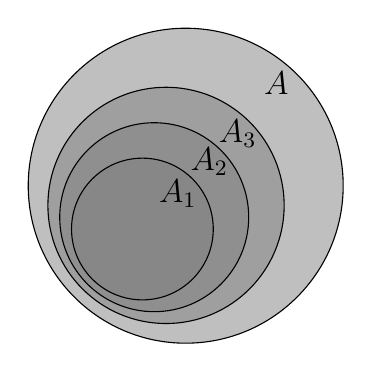
\begin{tikzpicture}
    \begin{scope}[fill opacity=0.5]
      \fill[gray] \firstcircle;
    \end{scope}
    \begin{scope}[fill opacity=0.5]
      \fill[gray] \secondcircle;
    \end{scope}
    \begin{scope}[fill opacity=0.5]
      \fill[gray] \thirdcircle;
    \end{scope}
    \begin{scope}[fill opacity=0.5]
      \fill[gray] \fourthcircle;
    \end{scope}

    \draw \firstcircle;
    \draw \secondcircle;
    \draw \thirdcircle;
    \draw \fourthcircle;

    \node at (0.45,0.45) {\large $A_1$};
    \node at (0.85,0.85) {\large $A_2$};
    \node at (1.21,1.21) {\large $A_3$};
    \node at (1.7,1.85) {\large $A$};

  \end{tikzpicture}
  \hskip 20pt
  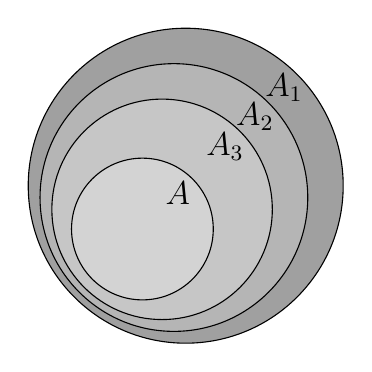
\begin{tikzpicture}
    \begin{scope}[fill opacity=0.75]
      \fill[gray] \fourthcircle;
    \end{scope}
    \begin{scope}[fill opacity=0.23]
      \fill[white] \firstcircle;
    \end{scope}
    \begin{scope}[fill opacity=0.23]
      \fill[white] \secondcircleb;
    \end{scope}
    \begin{scope}[fill opacity=0.23]
      \fill[white] \thirdcircleb;
    \end{scope}



    \draw \firstcircle;
    \draw \secondcircleb;
    \draw \thirdcircleb;
    \draw \fourthcircle;

    \node at (0.45,0.45) {\large $A$};
    \node at (1.05,1.05) {\large $A_3$};
    \node at (1.43,1.43) {\large $A_2$};
    \node at (1.8,1.8) {\large $A_1$};

  \end{tikzpicture}

  \label{fig-eventi-crescenti-decrescenti}
  \caption{eventi $A_n$ crescenti e decrescenti verso $A$}
\end{figure}


\medskip
\begin{teob}[\JPTh{2.3}]
  Siano $(\Omega, \Ac)$ spazio misurabile, e
  $\PP:\Ac \to [0,1]$ funzione additiva e tale che $\PP(\Omega) = 1$.
  Allora le seguenti affermazioni sono equivalenti:
  \begin{enumerate}
    \item $\PP$ è $\sigma$-additiva (ovvero $\PP$ è una probabilità)
    \item $A_n \in \Ac, \ A_n \downarrow    \varnothing     \implies \PP(A_n) \downarrow    0$
    \item $A_n \in \Ac, \ A_n \downarrow    A           \implies \PP(A_n) \downarrow    \PP(A)$
    \item $A_n \in \Ac, \ A_n \uparrow  \Omega      \implies \PP(A_n) \uparrow  1$
    \item $A_n \in \Ac, \ A_n \uparrow  A           \implies \PP(A_n) \uparrow  \PP(A)$
  \end{enumerate}
  Dai punti (3) e (5) si può dedurre lo \textit{scambio di limiti} $\PP(A) = \PP(\lim_{n} A_n) = \lim_{n} \PP(A_n)$.
\end{teob}
\smallskip
\begin{dimo}
  La dimostrazione si svolgerà così:
  \begin{enumerate}[label=(\alph*)]
    \item casi ovvi;
    \item (4) $\implies$ (5);
    \item (5) $\implies$ (1);
    \item (1) $\implies$ (5);
  \end{enumerate}
  \bigskip
  \begin{enumerate}[label=(\alph*)]
    \item
      \begin{itemize}
        \item (3) $\iff$ (5) per le leggi di De Morgan (complementarità);
        \item (2) $\iff$ (4) per le leggi di De Morgan (complementarità);
        \item (3) $\implies$ (2) e (5) $\implies$ (4) perché sono casi particolari.
      \end{itemize}
    \item (4) $\implies$ (5).
      Siano $A_n \in \Ac$ tali che $A_n \uparrow A$. Definiamo allora $B_n = A_n \cup A^C$. \\
      $B_{n+1} \supseteq B_n$. Allora $B_n \uparrow \Omega$ e dunque $\PP(B_n) \to 1$. Inoltre, vale:
      $$\bigcup\limits_{n} B_n = \bigcup\limits_{n} (A_n \cup A^C) = \left(\bigcup\limits_{n} A_n\right) \cup A^C = A \cup A^C = \Omega$$
      Passando alle probabilità:
      \begin{align*}
        \PP(B_n) &= \PP\left(A_n \cup A^C \right) \\
        &= \PP(A_n) + \PP \left(A^C\right) - \PP\left(A_n \cap A^C\right)\\
        &=  \PP(A_n) + \PP \left(A^C\right) \longrightarrow \PP(A) + \PP\left(A^C\right)
      \end{align*}
      Allora, sottraendo da entrambi i membri $\PP(A^C)$, si ha che $\PP(A_n) \to \PP(A)$.
    \item (5) $\implies$ (1).
      Siano $A_n \in \Ac$ tali che $ A_k \cap A_l = \varnothing \enspace \forall k \neq l.$ \\
      Definiamo dunque $B_n = \bigcup\limits_{k=1}^{n} A_k$.
      Questo garantisce che:
      $$B_n \subseteq B_{n+1} \quad \text{e} \quad B_n = \bigcup\limits_{k=1}^{n} B_k = \bigcup\limits_{k=1}^{n} A_k$$
      Possiamo quindi passare alla probabilità:
      \begin{align*}
        \PP(B_n) = \PP \left(\bigcup\limits_{k=1}^{n} A_k\right)
        &\implies \sum\limits_{k=1}^{n} (\PP(A_k)) = \PP\left(\bigcup\limits_{k=1}^{n} A_k\right)\\
        &\implies \sum\limits_{k=1}^{+\infty} (\PP(A_k)) = \PP \left( \bigcup\limits_{k=1}^{+\infty} A_k \right)
      \end{align*}

    \item (1) $\implies$ (5).
      Siano $A_n \uparrow A$, $A_n \in \Ac$.
      Si definisca la successione $B_n$ nel seguente modo:
      $$
      \begin{cases}
        B_1 = A_1\\
        B_2 = A_2 \setminus A_1 = A_2 \cap A_1^C\\
        \dots \\
        B_n = A_n \setminus A_{n-1}
      \end{cases}
      $$
      Visto che gli $A_n \uparrow A$ allora i $B_n$ risultano disgiunti e si può sfruttare la $\sigma$-additività, ripetendo la procedura del punto (c):
      $$\PP \left(\bigcup\limits_{n=1}^{+\infty} B_n \right) = \sum\limits_{n=1}^{+\infty} \PP(B_n) \qedhere$$
  \end{enumerate}
\end{dimo}

\bigskip
\begin{prop}[proprietà di subadditività]
  \index{subadditività}
  Data una successione numerabile di eventi $A_n \in \Ac \enspace \forall n$, vale la seguente disuguaglianza:
  $$\PP \left( \bigcup_{n=1}^{+\infty} A_n \right) \le \sum_{n=1}^{+\infty} \PP(A_n)$$
\end{prop}

Citiamo, inoltre, una disuguaglianza di verso opposto che tratta invece dell'intersezione finita di eventi.
\begin{prop}[disuguaglianza di Bonferroni]
  \index{Bonferroni, disuguaglianza di}
  Data una collezione finita di eventi $A_1, \dots, A_n \in \Ac$, si ha che:
  $$\PP \left( \bigcap_{i=1}^n A_i \right) \ge \sum_{i=1}^n \PP(A_i) - (n-1)$$
\end{prop}

\subsection{Probabilità su spazi campionari discreti} %qui Greg insiste sulla densità discreta che però c'è dopo
\begin{teo}[probabilità su spazi discreti \JPTh{4.1}]
Sia $\Omega$ discreto (ovvero con cardinalità al più numerabile).
  \begin{enumerate}
    \item $\PP$ su $(\Omega, \; 2^\Omega)$ è caratterizzata dai valori sugli \textit{atomi} (ossia elementi costituiti da un solo esito), cioè:
    $$p_\omega = \PP(\{\omega\}), \ \omega \in \Omega; \ \text{ infatti } \ \PP(A) = \sum\limits_{\omega \in A} (p_\omega) \quad \text{con } p:\Omega \to [0,1]$$
    \item Sia $p:\Omega \to [0,1]$. Allora:
      $$\exists! \; \PP: 2^\Omega \to [0,1]: \PP(\{\omega\}) = p_\omega \iff \begin{cases} p_\omega \geq 0 \quad \forall \omega \\[4pt] \sum\limits_{\omega \in \Omega} p_\omega = 1 \end{cases}$$
  \end{enumerate}
\end{teo}

\lezione{3}{15.03.17}
\begin{dimo}
  \Fixvmode
  \begin{enumerate}
    \item Siano $\PP:2^\Omega \to [0,1]$ e $A \in 2^\Omega, A \subseteq \Omega$. \\
  Allora $A = \bigcup\limits_{x \in A} \{x\}$ e essendo gli atomi eventi disgiunti, per $\sigma$-additività vale:
      $$\PP(A)  = \PP\left( \bigcup\limits_{x \in A} \{x\} \right) = \sum\limits_{x \in A} \PP( \{x\}) = \sum\limits_{x \in A} p_\omega$$
    \item \textbf{Dimostriamo ($\implies$)}:

      Per ipotesi $\exists! \, \PP:2^\Omega \to [0,1]$, si può allora porre $p_\omega = \PP(\{\omega\}) \in [0,1]$. Inoltre:
      $$\sum\limits_{\omega \in \Omega} p_\omega = \sum\limits_{\omega \in \Omega} \PP(\{\omega\}) = \PP(\bigcup\limits_{\omega \in \Omega} \{x\}) = \PP(\Omega) = 1$$
    \item[] \textbf{Dimostriamo ($\impliedby$)}:

      Sia $\PP:\Omega \to \RR$ tale che $p_\omega \geq 0$ e  $\sum\limits_{\omega \in \Omega} p_\omega = 1$.

      Posto $\PP(A) = \sum\limits_{\omega \in A} p_\omega$, allora $p_\omega = \PP(\{\omega\})$ ed è possibile mostrare che $\PP$ è una probabilità:
      \begin{itemize}
        \item $\PP(\Omega) = \sum\limits_{\omega \in \Omega} p_\omega = 1$;
        \item $\PP$ è $\sigma$-additiva, infatti dati $A_k \in 2^\Omega, \; k \in \NN, \; A_k \cap A_l = \varnothing \quad \forall k \neq l$:
          $$\PP\left( \bigcup\limits_{k=1}^{+\infty} A_k \right)
          = \sum\limits_{\omega \in \bigcup\limits_{k=1}^{+\infty} A_k} p_\omega
          = \sum\limits_{k=1}^{+\infty} \left[\sum\limits_{\omega \in A_k} p_\omega \right]
          = \sum\limits_{k=1}^{+\infty} \PP(A_k)$$
      \end{itemize}
    Allora $\exists! \, \PP:2^\Omega \to [0,1] \text{ tale che } \PP(\{\omega\}) = p_\omega$. \qedhere
  \end{enumerate}
\end{dimo}

\bigskip
\begin{ese}
  Dati $\Omega = \{0, 1, \dots, n\}$ e $p \in [0,1]$ fissato, si definisca la \emph{distribuzione binomiale} nel modo che segue:
  $$p_k = \binom{n}{k}p^k(1-p)^{n-k} \implies p_k \geq 0 \quad \forall k = 0, \dots, n$$
  Per lo sviluppo binomiale, o formula di Newton:
  $$\sum\limits_{k=0}^{n} \binom{n}{k}p^k (1-p)^{n-k} = [p + (1-p)]^n = 1$$
  La somma delle probabilità sugli atomi è dunque pari a 1, come richiesto a una probabilità.
\end{ese}

\medskip
\begin{ese}
  Dati $\Omega = \ZZ^+ = \{0, 1, 2, \dots\}$ e $\lambda > 0$, si definisca la \emph{distribuzione di Poisson} di parametro $\lambda$:
  $$p_k = (e^{-\lambda})\frac{\lambda^k}{k!} \implies \sum\limits_{k=0}^{+\infty} p_k
  = \sum\limits_{k=0}^{+\infty} (e^{-\lambda})\frac{\lambda^k}{k!}
  = (e^{-\lambda}) \sum\limits_{k=0}^{+\infty} \frac{\lambda^k}{k!} = e^{-\lambda}e^{\lambda} = 1$$
  Anche qui la probabilità totale è pari a 1.
\end{ese}

\medskip

\begin{defn}
  \index{spazio!di probabilità}
  Siano $(\Omega, \Ac)$ uno spazio misurabile e $\PP$ una probabilità su $\Ac$. \\
  La tripletta $\Dom$ è detta \textbf{spazio di probabilità}.
\end{defn}

\medskip
\begin{defn}
  \index{evento!quasi certo}
  \index{quasi certo (qc)!evento}
  \index{evento!improbabile}
  Dato uno spazio di probabilità $\Dom$, sia l'evento $A \in \Ac$. \\
  Se $\PP(A) = 0$, $A$ è detto \textbf{improbabile} (o trascurabile). Se invece $\PP(A) = 1$, A è detto \textbf{quasi certo}.
\end{defn}

\cleardoublepage
